\documentclass[conference]{IEEEtran}
\IEEEoverridecommandlockouts
% The preceding line is only needed to identify funding in the first footnote. If that is unneeded, please comment it out.
\usepackage{cite}
\usepackage{amsmath,amssymb,amsfonts}
\usepackage{algorithm, algorithmic}
\usepackage{graphicx}
\usepackage{textcomp}
\usepackage{xcolor}
\usepackage{hyperref}
\def\BibTeX{{\rm B\kern-.05em{\sc i\kern-.025em b}\kern-.08em
    T\kern-.1667em\lower.7ex\hbox{E}\kern-.125emX}}
\begin{document}

\title{Review: Basin-hopping Algorithm: Combining Global Stepping with Local Minimization*\\
{\footnotesize \textsuperscript{*}ECE 506 Project, Fall 2018}
\thanks{}
}

\author{\IEEEauthorblockN{Mustafa Salman}
\IEEEauthorblockA{\textit{Dept. of Electrical \& Computer Engineering} \\
\textit{University of New Mexico}\\
Albuquerque, NM \\
esalman@unm.edu}
}

\maketitle

\begin{abstract}
Stochastic algorithms are well-suited for optimization of complex and non-deterministic functions, but comes at a price of increased computational cost. Basin-hopping is a hybrid optimization algorithm implemented in the SciPy library. It combines the advantages of both stochastic and deterministic algorithms. In this work I presented a comparison of the performance between Basin-hopping algorithm and several other deterministic algorithms. Results show that Basin-hopping algorithm has better accuracy and robustness while having acceptable efficiency.
\end{abstract}

\begin{IEEEkeywords}
stochastic optimization, deterministic optimization, hybrid optimization, Basin-hopping
\end{IEEEkeywords}

\section{Introduction}

Typical deterministic optimization algorithms can optimize smooth continuous functions very well. Some of these algorithms can take advantage of gradients and Hessians (if exists) of such functions for faster convergence \cite{b1}. However, when it comes to continuous function with many local minima, these algorithms fall short. Furthermore, many real world problems are non-deterministic where these deterministic algorithms are not applicable. Stochastic algorithms are designed for solving such problems \cite{b3}.

Some stochastic algorithms apply random perturbations to the local minima at each iteration in order to traverse the solution space. Markov Chain Monte Carlo (MCMC) criteria are techniques for establishing a stationary distribution using the acceptable solutions \cite{b4}. The global minimum can be envisioned as the highest point of such a distribution. Stochastic algorithms are able to sample the possible solutions and eventually converge to a global minimum using the Metropolis criterion. Metropolis is just one of various types of MCMC techniques which are useful for sampling from a probability distribution when direct sampling is difficult \cite{b12}. These algorithms has shown promise in finding the solution of many difficult problems. However, there is no free lunch and this success comes at a price.

A major drawback of the stochastic algorithms is that in order to find the global minimum of complex functions, they need to sample a very high number of possible solutions and can only accept a fraction of those using a criterion such as Metropolis. This high computation cost is impractical in many circumstances, which has prevented widespread usage of these algorithms. There has been an attempt to formulate a class of algorithms which combine the best of both deterministic and stochastic algorithms.

The Scientific Computing Tools for Python (SciPy) library implements a hybrid  Basin-hopping algorithm \cite{b5}. The default implementation of this algorithm iteratively samples new candidate solutions from a uniform distribution, performs a local optimization and uses the Metropolis criterion in an acceptance test in order to reach global minima of a problem. The implementation offers various flexibilities such as using one of the many different deterministic algorithms for local minimization and customizing the random perturbation function among others. In this work I used this method to minimize several 2D continuous functions of varying complexity and compared the accuracy, efficiency and robustness of Basin-hopping with other deterministic functions.

\begin{figure}[htbp]
\centerline{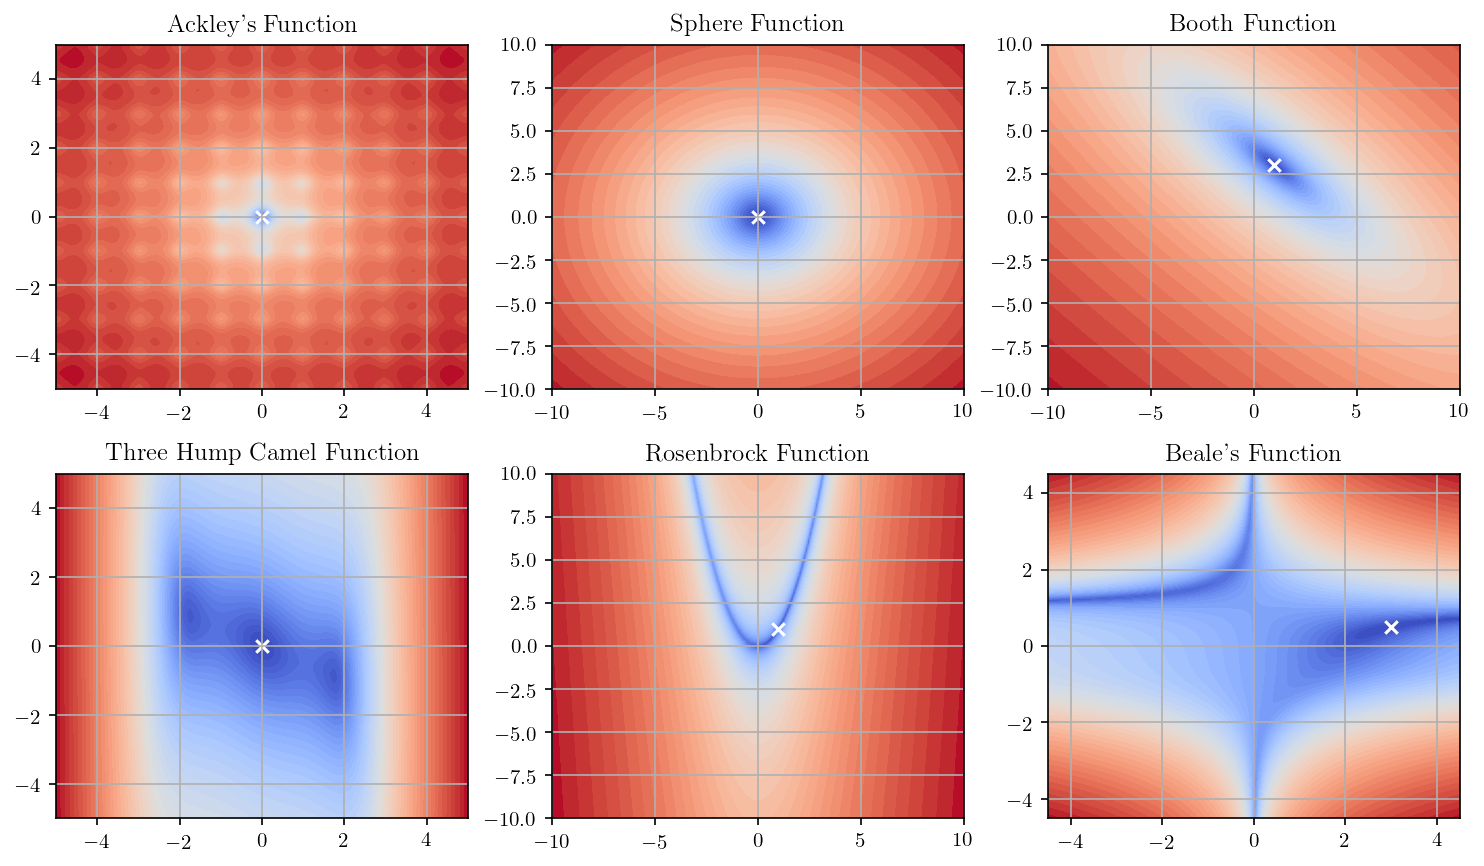
\includegraphics[width=.5\textwidth]{functions.png}}
\caption{Contour of various 2D continuous functions}
\label{functions}
\end{figure}

\section{Methods}

\begin{figure*}[htbp]
\centerline{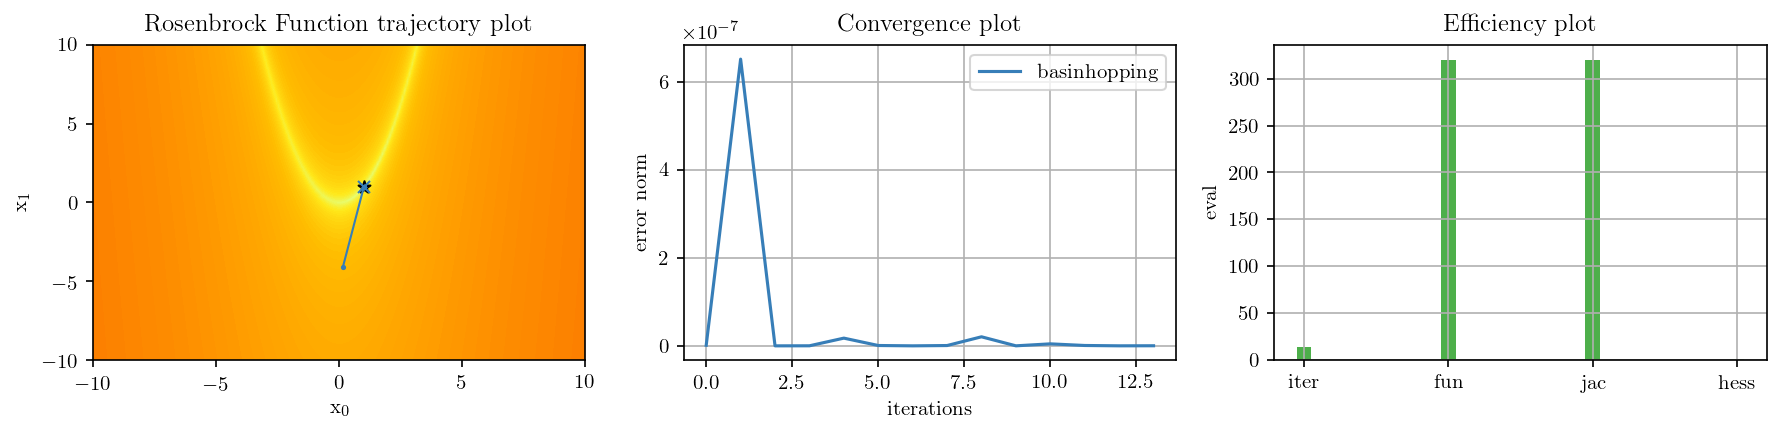
\includegraphics[width=\textwidth]{bfgs.png}}
\end{figure*}

\begin{figure*}[htbp]
\centerline{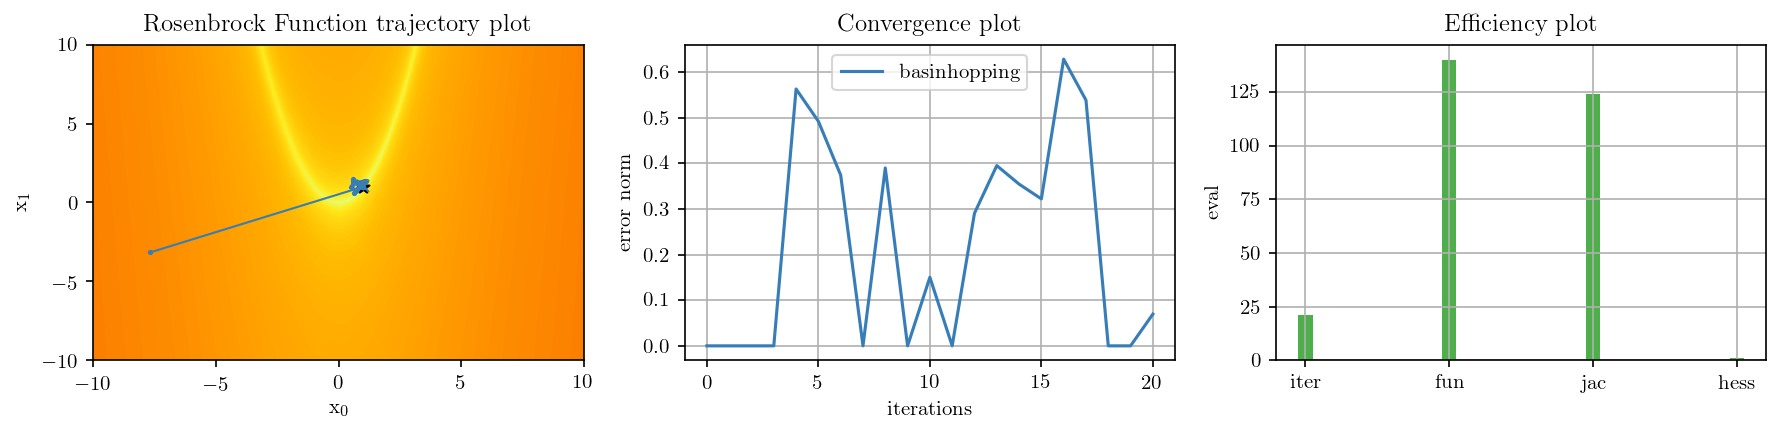
\includegraphics[width=\textwidth]{dogleg.png}}
\caption{Difference in the number of function evaluations when using \texttt{BFGS} or \texttt{dogleg} algorithm for local minimization in Basin-hopping. }
\label{dogleg}
\end{figure*}

\subsection{Continuous Testing Functions for Optimization}

I used an implementation of various continuous testing functions for optimization available on Github \cite{b3}. This module contains functions in one, two and multi-dimension. Each test function is implemented as a class with methods for calculating the cost, gradient and Hessian. Additional information such as the global minimum value and the function's domain are also provided. I found that out of 40 2D functions, 14 have all these methods implemented.

Some of the functions that I used are:

\begin{itemize}
    \item With many local minima: Ackley, Levy13
    \item Bowl-Shaped: Sphere
    \item Plate-Shaped: Booth, Matyas, McCormick
    \item Valley-Shaped: Three Hump Camel, Rosenbrock
    \item Steep Ridges/Drops: Absolute, Absolute Skewed, Easom, Beale, Goldstein-Price, Styblinski-Tang
\end{itemize}

\subsection{Basin-hopping Algorithm}

Basin-hopping is a stochastic algorithm which attempts to find the global minimum of a smooth scalar function of one or more variables \cite{b6}. It is presented in Alg. \ref{alg1}. The algorithm  implemented in the SciPy library was described by Wales and Doye \cite{b5}.

\subsubsection{Heuristics}
\begin{itemize}
	\item Random perturbation of the coordinates
	\item Local minimization
	\item Accept or reject the new coordinates based on the minimized function value
\end{itemize}

\begin{algorithm} % enter the algorithm environment
\caption{Basin-hopping $\min y = f(x)$ \cite{b6}} % give the algorithm a caption
\label{alg1} % and a label for \ref{} commands later in the document
\begin{algorithmic} % enter the algorithmic environment
    \STATE $i \leftarrow 0$
	\STATE $X_i \leftarrow \text{random initial point in variable space}$
	\STATE $Y_i \leftarrow \texttt{LOCALSEARCH}(X_i)$
    \WHILE{\texttt{STOP} \ \text{not satisfied}}
		\STATE $X_{i+1} \leftarrow \ \texttt{PURTURB}(Y_i)$
		\STATE $Y_{i+1} \leftarrow \ \texttt{LOCALSEARCH}(X_{i+1})$
        \IF{$f(Y_{i+1}) < f(Y_i)$}
            \STATE $i \leftarrow i+1$
        \ENDIF
    \ENDWHILE
\end{algorithmic}
\end{algorithm}

\begin{figure*}[htbp]
\centerline{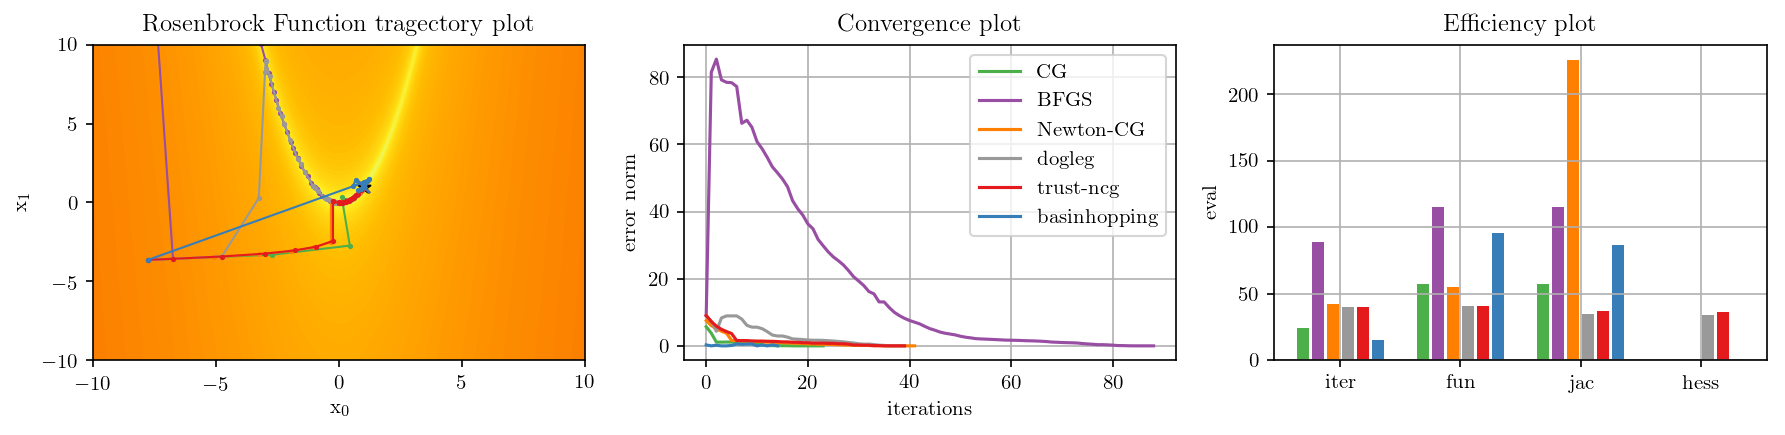
\includegraphics[width=\textwidth]{convergence.png}}
\caption{Trajectory for different algorithms, convergence and efficiency (number of iterations, function (cost, gradient and Hessian) evaluations for the Rosenbrock function)}
\label{convergence}
\end{figure*}

\subsubsection{Notes on the SciPy Implementation}

\begin{itemize}
	\item \texttt{LOCALSEARCH} uses the Broyden-Fletcher-Goldfarb-Shanno (\texttt{BFGS}) algorithm by default \cite{b13}. Using the \texttt{minimizer\_kwargs} parameter of Basin-hopping, it is possible to apply any \texttt{scipy.optimize.minimize} local minimization method and specify the gradient/Hessian as required. It is also possible to use a custom \textit{do nothing} function, along with a suitable \texttt{take\_step} callback, which may implement simulated annealing.
	\item A \texttt{callback} routine is implemented for each minima found. It can be used for tracking the performance of the algorithm.
	\item \texttt{PURTURB} uniformly samples a new $X_{i+1}$ from $[X_{i}-\texttt{stepsize}, X_{i}+\texttt{stepsize}]$ in each dimension. \texttt{stepsize} is adjusted automatically by the Basin-hopping algorithm, but can also be passed as a parameter. The \texttt{take\_step} callback can replace the default step-taking routine.
	\item The acceptance test uses the Metropolis criterion of standard Monte Carlo algorithm. Steps are always accepted if $f(X_{i+1}) < f(X_i)$. Otherwise, they are accepted with probability 
	$$exp( -\frac{f(X_{i+1}) - f(X_i)}{T} )$$
	Where $T$ is the \textit{temperature} used in the Metropolis criterion. If $T=0$, then all steps that increase the function value are rejected. An \texttt{accept\_test} callback is also implemented for defining custom acceptance test.
	\item \textit{Other parameters:} An optional \texttt{interval} parameter is available which determines how often \texttt{stepsize} is updated. The \texttt{niter\_success} parameter stops the run if global minimum candidate remains the same for this number of iterations.
	\item It is advised that both \texttt{T} and \texttt{stepsize} should be chosen based on the typical difference between the local minima of the function being optimized.
\end{itemize}

\subsection{Experiments}

I performed the following experiments to understand how the Basin-hopping algorithm works, and how it fares compared to the other deterministic algorithms implemented in SciPy.

\subsubsection{Using different local optimization methods}

For this experiment I looked at how Basin-hopping performs for different algorithm choices for the \texttt{LOCALSEARCH} routine.

\subsubsection{Cross-validation for \texttt{T} \& \texttt{stepsize}}

For this experiment I tried to find the optimal \texttt{T} and \texttt{stepsize} parameters for minimizing the 2D \textit{Rosenbrock} function. \texttt{T} was varied logarithmically between .01 and 100; and \texttt{stepsize} was varied linearly between 0.1 and 3.0. A grid search was performed for each pair of (\texttt{T}, \texttt{stepsize}). For each pair, the experiment was repeated 100 times with random initialization of the starting value. The mean number of function (cost, gradient and Hessian) evaluations and error norms were reported.

\subsubsection{Comparing Accuracy \& Efficiency}

For this experiment, I looked at how Basin-hopping fares in terms of convergence and efficiency compared to several deterministic algorithms. The algorithms used for comparison were: conjugate gradient (\texttt{CG}), \texttt{BFGS}, \texttt{Newton-CG}, \texttt{dogleg} and trust-region Newton-CG (\texttt{trust-ncg}). These algorithms are implemented in the \texttt{scipy.optimize.minimize} routine. \texttt{CG}, \texttt{BFGS} and \texttt{Newton-CG} only require the gradient of the function. \texttt{dogleg} and \texttt{trust-ncg} require the Hessian, \texttt{dogleg} requires the Hessian to be positive semi-definite in addition. I used these methods to optimize different functions from the same starting point. The convergence (error norm vs iterations) and number of function evaluations were noted.

\subsubsection{Comparing Robustness}

For this experiment, I used all of the above methods to optimize different functions, each one a number of times (100) with random initializations. The mean and standard deviation of the average number of function (cost/gradient/Hessian) evaluations and error norm were noted.

\begin{figure}[htbp]
\centerline{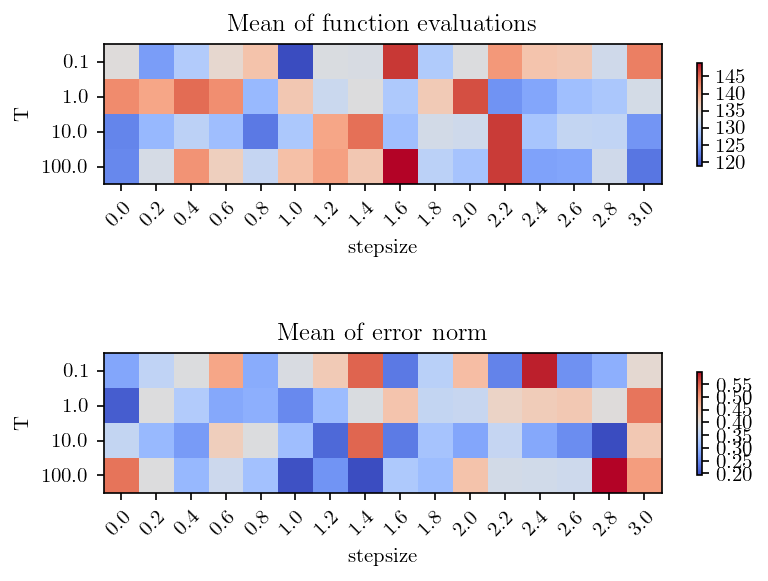
\includegraphics[width=.5\textwidth]{T_stepsize.png}}
\caption{Basin-hopping performance for different pairs of (\texttt{T}, \texttt{stepsize})}
\label{T_stepsize}
\end{figure}

\section{Results}

Some of the function contours used for performing the experiments are depicted in Fig. \ref{functions}

\begin{figure*}[htbp]
\centerline{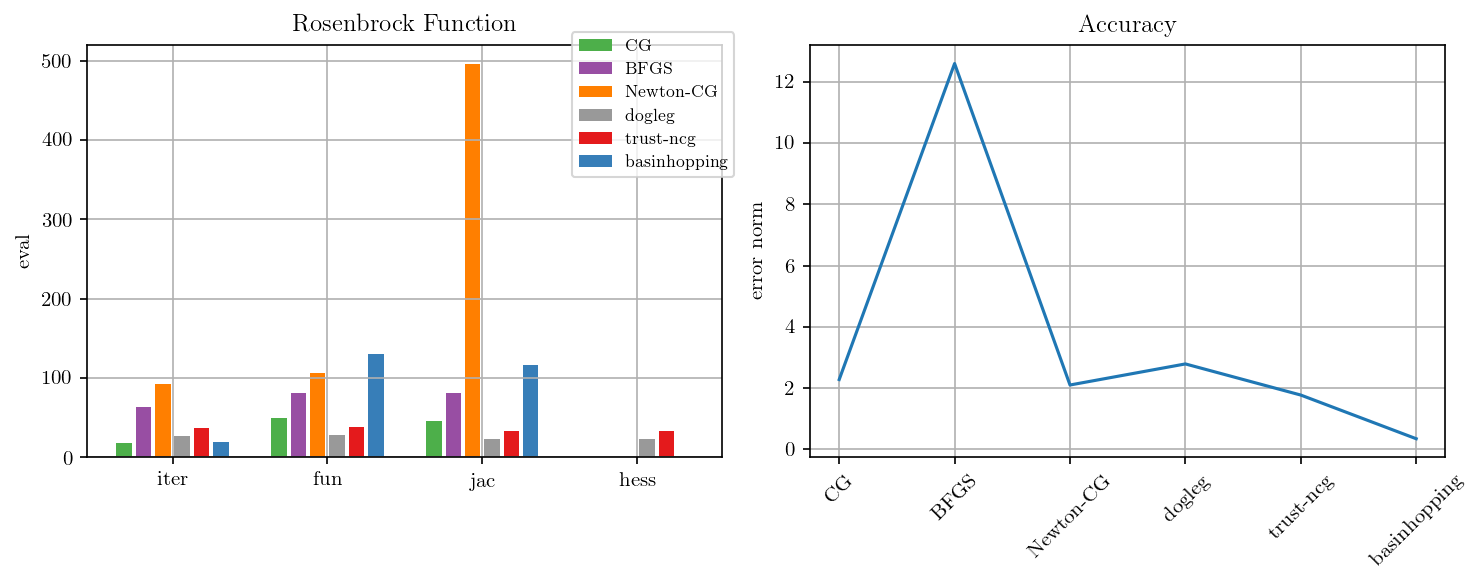
\includegraphics[width=\textwidth]{robust.png}}
\caption{Average function evaluation and error norm over 100 repetitions of each algorithm at minimizing the Rosenbrock function}
\label{robust}
\end{figure*}

\subsection{Using different local optimization methods}

Fig. \ref{dogleg} shows the efficiency (and convergence) of Basin-hopping using \texttt{BFGS} and \texttt{dogleg} for the \texttt{LOCALSEARCH} step. \texttt{dogleg} requires fewer function evaluations because of using the the Hessian for faster convergence. However, \texttt{BFGS} shows better accuracy at minimizing functions with many local minima.

\subsection{Cross-validation for \texttt{T} \& \texttt{stepsize}}

Fig. \ref{T_stepsize} shows the performance of Basin-hopping for different pairs of (\texttt{T}, \texttt{stepsize}). It is difficult to choose a \texttt{T} from this plot, although lower \texttt{stepsize} seems to result in less error.

\subsection{Comparing Accuracy \& Efficiency}

Fig. \ref{convergence} shows the convergence for various algorithm at minimizing the Rosenbrock function. It shows that Basin-hopping with \texttt{dogleg} needs less than 100 function cost and gradient evaluations to converge. This is quite low compared to typical stochastic algorithms. It also requires the least stochastic iterations than any other method.

\subsection{Comparing Robustness}

Fig. \ref{robust} shows the mean number of iterations, function (cost, gradient and Hessian) evaluations and error norms over 100 repetitions of each algorithm at minimizing the Rosenbrock function. The numbers hover around 100 for Basin-hopping, which is feasible considering that it results in the lowest average error norm.

\section{Discussion}

I tried to minimize 14 functions (some of them quite nasty) using the deterministic algorithms available from SciPy, and a hybrid algorithm (Basin-hopping). There are 26 more functions in the Github repository which do not implement the gradient or Hessian. All of the SciPy optimization routines implement a \texttt{callback} method at each iteration. I used this method to track the local minima and error norm.

Basin-hopping error is lower, but function evaluation is higher when using the gradient-based \texttt{BFGS} for local minimization compared to the Hessian-based \texttt{dogleg}. Compared to the deterministic algorithms,  Basin-hopping with \texttt{dogleg} is more efficient but less accurate, and Basin-hopping with \texttt{BFGS} is the opposite. The former can beat deterministic algorithms at minimizing smooth functions, and the latter can do the same at minimizing functions with rough surfaces. It is easy to break the deterministic algorithms using a starting point outside of the suitable domain. For instance, \texttt{BFGS} blows up but Basin-hopping appears very reliable for minimizing the Beale function.

Following are the analyses of some common errors encountered when performing the experiments.
\begin{itemize}
	\item "Desired error not necessarily achieved due to precision loss": occurs due to the inability to solve the minimization subproblem.
	\item "free variable 'gfk' referenced before assignment in enclosing scope": occurs in Newton-CG due to bad starting points.
	\item "array must not contain infs or NaNs": occurs in \texttt{trust-ncg} when the gradient calculation blow up. Typically caused by bad starting points outside the function domain.
	\item "A linalg error occurred, such as a non-psd Hessian": happens in \texttt{dogleg}.
	\item "A bad approximation caused failure to predict improvement": happens in \texttt{trust-ncg}.
\end{itemize}

\subsection{Future Directions}

I found the "Continuous Testing Functions for Optimisation" Github repository very useful. It saved a lot of time at the start of the project. However, not all the functions in this module have the gradient and Hessian implemented. It will be a good idea to contribute these implementations in this repository.

Further experimentation with the Basin-hopping options is necessary in order to find suitable \texttt{T} and \texttt{stepsize}. In addition, how the algorithm adjusts the \texttt{stepsize} using the \texttt{interval} parameter is also worth a look.

For this experiment I did not look at the timing or memory consumption, as all the SciPy routines were very fast at solving the continuous functions. Even the robustness experiment with 14 functions, 6 different algorithms and 100 repetitions only took a few seconds even without parallelization. It will be worth looking at the timing and memory performance, especially for solving non-deterministic problems. There is a nice Python module consisting of such problems and stochastic algorithms called NiaPy \cite{b8}.

Another important measure of performance is the optimization status returned by the SciPy \texttt{mimimize} routine. It tells us if the solution actually converged or not. In the robustness experiment, at times the algorithms did not converge but the error norm and function evaluation were still taken into account. The status should also be taken into account for better assessment of the robustness.

\vfill
\pagebreak

\begin{thebibliography}{00}
\bibitem{b1} J. Nocedal and S. J. Wright, Numerical optimization, 2nd ed. New York: Springer, 2006.
\bibitem{b2} D. P. Kroese, T. Taimre, and Z. I. Botev, Handbook of Monte Carlo Methods. John Wiley \& Sons, 2013.
\bibitem{b3} M. Herman, “Simulated Annealing \& the Metropolis Algorithm: A Parameter Search Method for Models of Arbitrary Complexity,” p. 14.
\bibitem{b4} R. Christensen, W. Johnson, A. Branscum, and T. E. Hanson, Bayesian Ideas and Data Analysis: An Introduction for Scientists and Statisticians, 1 edition. Boca Raton, FL: CRC Press, 2010.
\bibitem{b5} D. J. Wales and J. P. K. Doye, “Global Optimization by Basin-Hopping and the Lowest Energy Structures of Lennard-Jones Clusters Containing up to 110 Atoms,” The Journal of Physical Chemistry A, vol. 101, no. 28, pp. 5111–5116, Jul. 1997. Available: \href{https://pubs.acs.org/doi/10.1021/jp970984n}{https://pubs.acs.org/doi/10.1021/jp970984n}
\bibitem{b6} B. Olson, I. Hashmi, K. Molloy, and A. Shehu, “Basin Hopping as a General and Versatile Optimization Framework for the Characterization of Biological Macromolecules,” Advances in Artificial Intelligence, 2012. [Online]. Available:
\href{https://www.hindawi.com/journals/aai/2012/674832/}{https://www.hindawi.com/journals/aai/2012/674832/}. [Accessed: 14-Dec-2018].
\bibitem{b7} L. Marris, Continuous Test Functions for Optimisation. Available: \href{https://github.com/lukemarris/ctf}{https://github.com/lukemarris/ctf}. 2018.
\bibitem{b8} NiaOrg, NiaPy: Python micro framework for building nature-inspired algorithms. .
\bibitem{b10} “scipy.optimize.basinhopping — SciPy v0.18.1 Reference Guide.” [Online]. Available: \href{https://docs.scipy.org/doc/scipy-0.18.1/reference/generated/scipy.optimize.basinhopping.html}{https://docs.scipy.org/doc/scipy-0.18.1/reference/generated/scipy.optimize.basinhopping.html}. [Accessed: 14-Dec-2018].
\bibitem{b11} “scipy.optimize.minimize — SciPy v0.18.1 Reference Guide.” [Online]. Available: \href{https://docs.scipy.org/doc/scipy-0.18.1/reference/generated/scipy.optimize.minimize.html#scipy.optimize.minimize}{https://docs.scipy.org/doc/scipy-0.18.1/reference/generated/scipy.optimize.minimize.html\#scipy.optimize.minimize}. [Accessed: 14-Dec-2018].
\bibitem{b12} W. K. Hastings, “Monte Carlo sampling methods using Markov chains and their applications,” Biometrika, vol. 57, no. 1, pp. 97–109, Apr. 1970.
\bibitem{b13} R. Fletcher, Practical methods of optimization, 2nd ed. Chichester ; New York: Wiley, 1987.
\end{thebibliography}
\vspace{12pt}

\end{document}

